%----------------------------------------------------------
% PACKAGES AND THEMES
%----------------------------------------------------------
\documentclass[aspectratio=169,xcolor=dvipsnames,handout]{beamer}

\usetheme{Darmstadt}
\usecolortheme{seahorse}

\usepackage[hangul]{kotex}
\usepackage{hyperref}
\usepackage{graphicx, array, adjustbox, makecell}
\usepackage{booktabs, multicol, multirow}
\setbeamercovered{transparent}

%----------------------------------------------------------
% TITLE PAGE
%----------------------------------------------------------
\title{노동조합과 경영자조직 및 정부}
\subtitle{노사관계의 이론과 실제}
\author{오성재}
\institute[CNU]
{\relax
    충남대학교 경제학과\\
}
\date{2024년 9월 23일}

%----------------------------------------------------------
\begin{document}
%----------------------------------------------------------

\frame{\titlepage}

\begin{frame}{목차}
    \small
    %아래 둘 중 하나만 쓸 것
    \tableofcontents[hideallsubsections]
    %\tableofcontents
\end{frame}

\section{노동조합의 이데올로기, 역할 및 기능}

\subsection{노동조합의 이데올로기}

\begin{frame}[allowframebreaks]{이념별 노동조합의 종류}
    \begin{itemize}
        \item 노동조합의 공통적인 특징: 
        \begin{itemize}[<+->]
            \item 노동조합은 근로자가 집단적으로 단결하여 요구조건을 달성하고자 자주적으로 조직한 항구적 단체
        \end{itemize}
        \item 노동조합은 국가별로 상이:
        \begin{itemize}[<+->]
            \item 각 국가가 처한 역사적 상황과 지배적인 사상에 따라 노동조합의 이데올로기는 차이를 보임
        \end{itemize}
    \end{itemize}
    \framebreak\relax
    \begin{enumerate}
        \item 혁명적 노동조합주의 (revolutionary unionism)
        \begin{itemize}[<+->]
            \item 정부와 자본주의체제를 전복시키고 공산주의나 무정부주의 등 새로운 사회를 건설하는 것을 목표
            \item 정치적인 구호나 주장, 유사시 동원 및 투쟁 중심
            \item 예: 프랑스에서 가장 큰 노조 조직인 프랑스노동총연맹 (CGT) 등
        \end{itemize}
        \framebreak\relax
        \item 사회적 노동조합주의 (social unionism)
        \begin{itemize}[<+->]
            \item 자본주의적 자유 이념보다는 사회적 합의 이념을 중시 
            \item 사회적 복지 국가를 지향 사회체제의 점진적 변혁을 기도
            \item 단체협상과 같은 경제적 수단과 의회를 통한 로비와 입법과 같은 정치적 수단을 병행.
            \item 예: 진보주의적인 성격이 강한 핀란드, 스웨덴의 LO
        \end{itemize}
        \framebreak\relax
        \item 경제적 노동조합주의 (business unionism)
        \begin{itemize}[<+->]
            \item 자본주의 체제를 인정하고 시장경제체제하에서 노동조합원의 임금이나 노동조합의 개선을 목표 
            \item 입법을 통한 정치적인 수단보다는 단체협상 등의 순수한 경제적 수단을 중시
            \item 노동계층 전체보다 조합원들만의 경제적인 지위향상에 전력을 기울임
            \item 예: 미국의 AFLCIO, 일본의 '렌고' 등
        \end{itemize}
    \end{enumerate}
\end{frame}

\subsection{노동조합의 역할}

\begin{frame}[allowframebreaks]{노동조합의 주요 역할}
    \begin{enumerate}[<+->]
        \item 조직화역할 (organizing model)
        \begin{itemize}[<+->]
            \item 노동조합의 존립과 발전을 위하여 신규 노조원을 조직하고 그들을 동원·선동하여 자신들의 주장을 관철하는 역할
            \item 조합원의 다양한 요구조건을 민주적으로 수용하고 또 지속적으로 조직·관리·동원하여 노동조합의 영향력을 유지하여야 
        \end{itemize}
        \framebreak\relax
        \item 서비스역할 (service model)
        \begin{itemize}[<+->]
            \item 노조는 조합원을 위하여 각종 서비스 제공
            \item 피보험자가 보험수수료를 납부하고 보험사고 발생 시 이에 대한 보상을 받는 것과 유사
            \begin{itemize}[<+->]
                \item 노조원이 조합비를 납부하고 고용안정이나 임금인상 등의 서비스 혜택을 받음
            \end{itemize}
            \item 노조의 서비스가 노조원의 욕구를 만족시키면 노조원의 지속적인 지지를 받지만 그렇지 못하면 외면
            \begin{itemize}[<+->]
                \item 노동자와 노조가 당면한 문제를 조합원들의 참여와 활동으로 해결, 노조는 존폐를 결정
            \end{itemize}
        \end{itemize}
    \end{enumerate}
\end{frame}

\section{노동조합의 조직형태}

\subsection{노조 조직형태의 분류}

\begin{frame}[allowframebreaks]{직업별 노동조합 (craft union)}
    \begin{itemize}[<+->]
        \item 동일한 직능을 갖는 숙련노동자들이 자신들의 경제적 이익을 확보하기 위하여 만든 조직체
        \begin{itemize}[<+->]
            \item 직업독점과 노동력의 공급제한
        \end{itemize}
        \item 산업화 초기의 노동조합 형태로 직능별 또는 직종별 조합이라고 불림
        \item 인쇄공조합, 선반공조합, 목공조합, 전기공 조합 등
        \item 예: 전국교직원노동조합, 대한민국공무원노동조합총연맹
        \framebreak\relax
        \item 장점
        \begin{itemize}[<+->]
            \item 동일한 직종을 대상으로 하기 때문에 단체교섭 사항과 내용이 명확  
            \item 조합원의 유대의식이 강해 조직의 단결력이 공고하며 어용화될 가능성 적음
            \item 실업자라 하더라도 조합의 가입이 가능하고 동종 조합원의 실업 예방
        \end{itemize}
        \item 단점
        \begin{itemize}[<+->]
            \item 숙련노동자 중심의 배타적이고 독점적 조직이기 때문에 조직대상이 한정 
            \item 미숙련노동자 등의 반발을 불러일으켜 전체 노동자의 분열 가능
            \item 조합의 자주성을 얻을 수 있으나 사용자와의 관계가 희박함
        \end{itemize}
    \end{itemize}
\end{frame}

\begin{frame}[allowframebreaks]{일반 조합 (general union)}
    \begin{itemize}[<+->]
        \item 숙련이나 직능, 산업과는 관계없이 모든 노동자들이 가입자격을 가진 전국적 단일노동조합
        \item 초기 직업별 조합에서 배제된 미숙련 노동자와 단순노동 종사자를 대상으로 조직
        \item 안정된 고용의 확보, 노동시간의 최고한도 규제, 임금의 최저한도 규제 등을 요구
        \item 주요 활동내용은 입법활동을 통한 최저생활 확보
        \framebreak\relax
        \item 특징
        \begin{itemize}[<+->]
            \item 미숙련 노동자 중심의 조합원들을 결속시키기 위해 중앙집권적 관료제 불가피
            \item 이질적인 조합원간 이해관계의 조정 및 통합의 어려움
            \item 단체교섭기능 약화 가능성
        \end{itemize}
        \item 예: 미국의 노동기사단 (Knights of Labor), 한국노총 산하 연합노조, 전국여성노동조합연맹 등
    \end{itemize}
\end{frame}

\begin{frame}{산업별 조합 (industrial union)}
    \begin{itemize}[<+->]
        \item 동일산업에 종사하는 모든 근로자가 하나의 노동조합을 구성하는 조직형태
        \item 직업별 조합이나 일반조합보다 늦게 발달
        \item 장점
        \begin{itemize}[<+->]
            \item 동일산업이 조직대상: 거대한 조직, 단결력 강화,  커다란 압력단체 기능
            \item 자본의 집중화에 대응하여 교섭력을 가질 수 있고, 산업내 근로조건의 통일 가능
        \end{itemize}
        \item 단점
        \begin{itemize}[<+->]
            \item 각 산업별 조직의 내부에서 직종간의 이해대립과 반목 초래 가능
            \item 위와 같은 경우 조직의 큰 힘을 발휘할 수 없음
        \end{itemize}
        \item 경제위기 이후 기업별 노조의 산별 노조화가 활발
        %\item 예: 전국전력노동조합·전국금융산업노동조합·전국담배인삼노동조합 전국우정노동조합 (이상 한국노총 소속) 전국대학노동조합·전국금속산업노동조합·보건의료노동조합 (이상 민주노총 소속)
    \end{itemize}
\end{frame}

\begin{frame}[allowframebreaks]{기업별 조합 (enterprise union)}
    \begin{itemize}[<+->]
        \item 동일한 기업에 종사하는 노동자로서 조직되는 노동조합
        \item 생성원인
        \begin{itemize}[<+->]
            \item 노동자 의식이 계급의식 등 횡단적 연대의식을 뚜렷이 갖지 않는 환경에서 조직
            \item 단위기업간의 시설규모나 지불능력의 차이 등 기업격차가 심한 곳에서 많이 나타남
            \item 정부 주도의 경제개발로 거대기업이 먼저 생성되는 환경에서 발생 (주로 후발공업국)
        \end{itemize}
        \framebreak\relax
        \item 장점: 노사협력이 용이
        \item 단점: 노동시장에 대한 영향력 미비, 조직 역량 미흡
        \begin{itemize}[<+->]
            \item 기업 내 각 직종간 요구조건을 공평하게 처리하기 어려움
            \item 기업 내 구성원만이 조직대상: 조합원 수가 적어 뚜렷한 자기기능 발휘 어려움
            \item 다른 노동조합의 형태보다 사용자의 영향력이 상대적으로 커 어용화 될 가능성 
        \end{itemize}
        \item 일본에서 크게 발달: 종신고용제, 노동시장의 이중구조, 家 중심의 사고방식
        \item 예: 일본 도요타자동차 노조, 쌍용자동차노동조합, 미래에셋대우노동조합
    \end{itemize}
\end{frame}

\section{노동조합의 설립과 운영}

\subsection{노조의 설립요건, 결격사유 및 신고주의}

\begin{frame}[allowframebreaks]{노동조합의 정의}
    \begin{block}{노동조합}
        근로자가 주체가 되어 자주적으로 단결하여  근로조건의 유지·개선 기타 근로자의 경제적·사회적 지위의 향상을 도모함을 목적으로 조직하는 단체 또는 연합단체
    \end{block}
    \begin{enumerate}[<+->]
        \item 근로자 주체 조직: 근로자 이외의 제3자, 특히 사용자로부터의 독립성을 유지하여야 함
        \item 자주적으로: 근로자 스스로의 의사에 의하여 조직하고 운영에 있어 사용자는 물론 행정관청, 정당 또는 종교 등으로부터 독립해야 함
    \framebreak\relax
        \item 근로조건의 목적으로: 근로조건의 유지 개선이라는 경제적 측면을 주목적으로 함. 또한 부차적으로 공제·복리 등의 사업을 하는 것도 가능
        \item 조직단체 또는 연합단체: 단위노조 또는 단위노동조합의 단체들이 결합한 조직체
    \end{enumerate}
    \begin{itemize}[<+->]
        \item 우리나라는 노동조합 설립 시 신고주의 채택
        \begin{itemize}[<+->]
            \item 행정관청에 설립신고서와 규약을 제출 신고하고 신고증을 교부 받아야 함
            \item 설립신고서가 반려되어 `법외 노조'가 되는 경우도 있음. 
        \end{itemize}
    \end{itemize}
\end{frame}

\subsection{노동조합의 운영과 노동조합 규약}

\begin{frame}{노동조합 규약}
    \begin{itemize}[<+->]
        \item 노동조합의 민주적 운영에 초석이 될 수 있는 민주적 노동조합규약 필수적
        \item 노동조합 규약의 요소
        \begin{itemize}[<+->]
            \item 노동조합 규약, 명칭, 목적과 사업, 주된 사무소의 소재지
            \item 조합원에 관한 사항, 소속된 연합단체가 있는 경우에는 그 명칭
            \item 대의원회를 두는 경우에는 대의원회에 관한 사항, 회의에 관한 사항
            \item 대표자와 임원에 관한 사항, 조합비 기타 회계에 관한 사항
            \item 규약변경에 관한 사항, 해산에 관한 사항
            \item 쟁의행위와 관련된 찬반투표 결과의 공개, 투표자 명부 및 투표용지 등의 보존 열람
            \item 대표자와 임원의 규약위반에 대한 탄핵에 관한 사항
            \item 임원 및 대의원의 선거절차에 관한 사항, 규율과 통제에 관한 사항
        \end{itemize}
    \end{itemize}
\end{frame}


\subsection{노동조합의 가입과 탈퇴}

\begin{frame}{조합에의 가입}
    \begin{itemize}[<+->]
        \item 헌법 제33조에서 노동3권 (단결권, 단체교섭권 및 단체행동권) 인정
        \item 자유의사에 의하여 조합에 가입할 자유가 보장되어 있음 (노동조합 및 노동관계조정법 제5조)
        \item 근로자들은 자유의사에 의하여 조합에 가입할 자유가 보장되어야 함
    \end{itemize}
\end{frame}

\begin{frame}{숍 (shop) 제도}
    \begin{itemize}[<+->]
        \item 노동조합의 가입과 취업을 관련시키는 것으로서 노동조합의 규모와 통제력을 좌우할 수 있는 제도
        \begin{itemize}[<+->]
            \item open shop: 노동조합의 가입 여부에 관계없이 채용할 수 있는 제도, 무임승차 문제
            \item closed shop: 채용 또는 충원 시 조합원 중에서만 고용하도록 하는 제도
            \item union shop: 취업 후에 일정기간이 경과하면 자동적으로 노조에 가입하게 되는 제도
            \item agency shop: 조합가입 여부에 관계없이 노동조합이 모든 종업원에게 조합회비를 징수하는 제도
            \item preferential shop: 채용에 있어 노동조합원에게 우선순위를 부여하는 제도
            \item maintenance of membership shop: 조합원이 되면 일정기간 동안 조합원의 지위를 유지하여야 하는 제도
        \end{itemize}
        \item 우리나라 closed shop은 부당노동행위로 금지
    \end{itemize}
\end{frame}

\begin{frame}{조합원 지위의 상실}
    \begin{itemize}[<+->]
        \item 조합원 지위 상실 조건
        \begin{itemize}[<+->]
            \item 조합원의 사망
            \item 조합원이 승진 또는 승격
            \item 기업별 조합의 경우 퇴직 또는 해고  (단, 해고의 효력을 다투는 자는 제외)
            \item 탈퇴
            \item 제명
        \end{itemize}
    \end{itemize}
\end{frame}

\section{노동조합의 추세와 현황}

\subsection{한국 노조의 추세와 현황}

\begin{frame}{연도별 노동조합 현황}
    \begin{itemize}[<+->]
        \item 1987년 이후 민주화의 분위기 속에서 노동조합 가입자 수, 조직률, 단위 조직수 등 증가
        \item 1989년 최고점에 도달한 후 계속적으로 하락하는 추세였음
        \item 2011년 복수노조 시행 등 영향으로 노동조합수, 노동조합원수 증가
        \item 2017년 문재인정부 등장후 노동조합 수, 조합원수 및 조직률 다시 증가 추세
    \end{itemize}
\end{frame}

\begin{frame}
\centering
\begin{figure}
    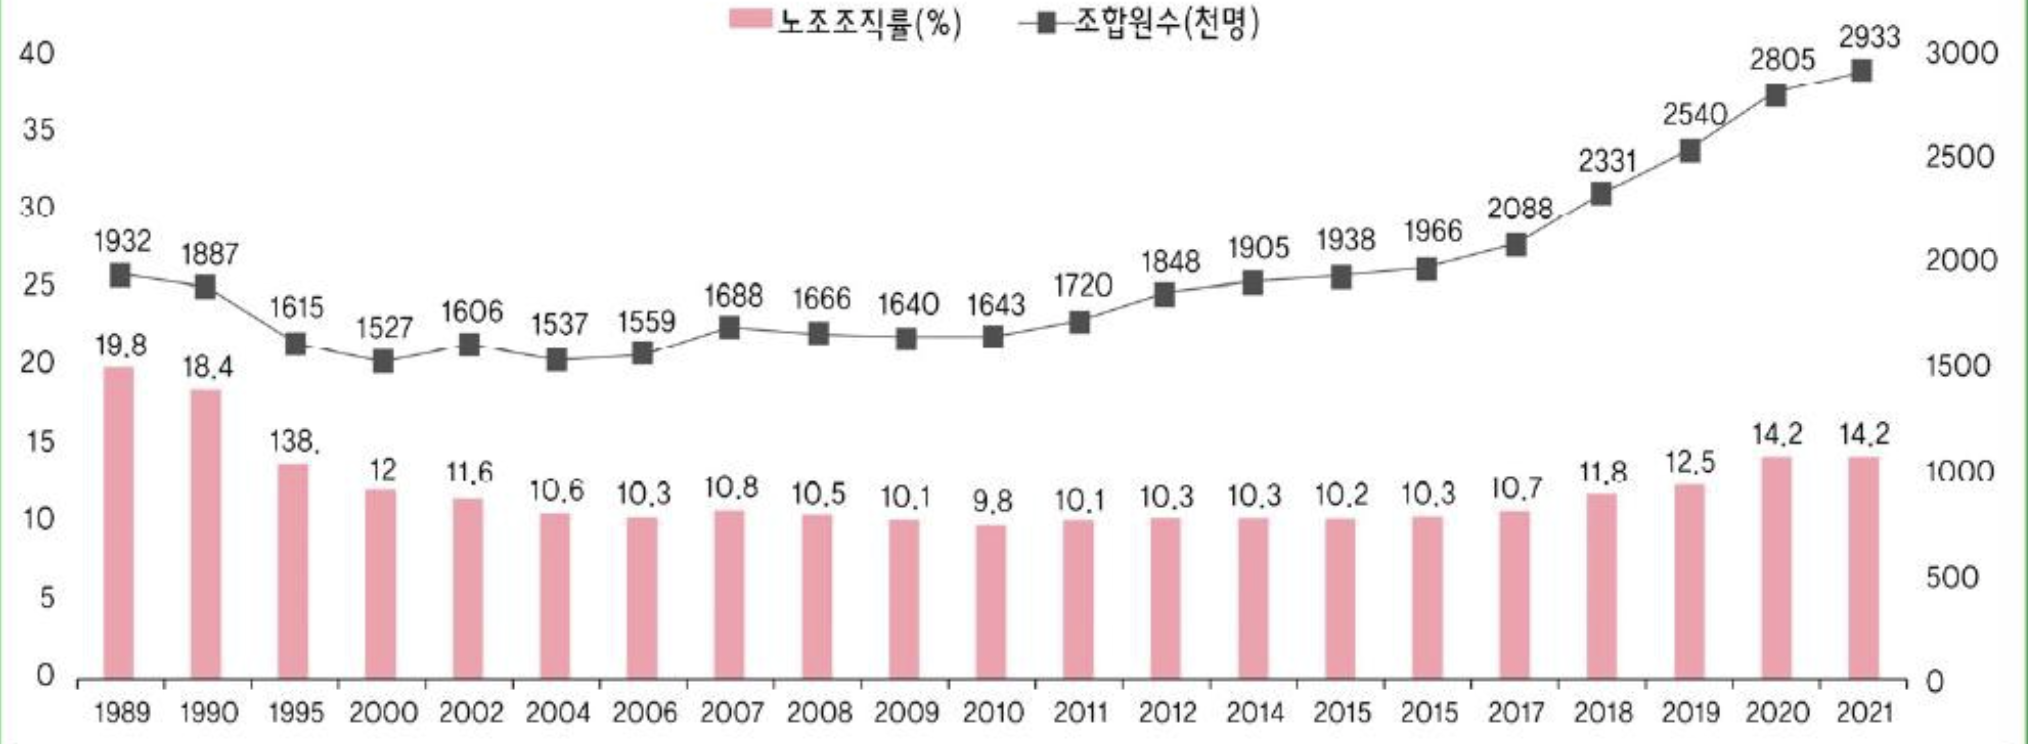
\includegraphics[width=.8\textwidth]{pic/연도별노조조직률및조합원수추이.png}
    \caption{연도별 노조 조직률 및 조합원수 추이}
\end{figure}
\end{frame}

\begin{frame}{사업체 규모별 노동조합 현황}
    \begin{itemize}[<+->]
        \item 중소기업 근로자들이 상대적으로 고용이 불안정하고 임금 등 근로조건 수준이 낮으나 대기업 근로자들에 비하여 노동조합에 의해 더 적게 보호 받고 있는 상황
    \end{itemize}
    \scriptsize
    \begin{table}
        \centering
        \resizebox{.8\textwidth}{!}{\relax
            \begin{tabular}{c|c|c|c|c}
\toprule
\textbf{구분} & \textbf{30명 미만} & \textbf{30~99명} & \textbf{100~299명} & \textbf{300명 이상} \\ \midrule
\textbf{임금근로자수(명)} & 11,978,000 & 3,968,000 & 2,046,000 & 2,879,000 \\ \hline
\textbf{조합원수(명)} & 25,170 & 63,207 & 212,586 & 1,333,530 \\ \hline
\textbf{조직률} & 0.2\% & 1.6\% & 10.4\% & 46.3\% \\ \bottomrule
\end{tabular}

        }
        \\
        \raggedright\relax % 왼쪽 정렬
        \caption{사업체 규모별 노동조합 조직 현황}
    \end{table}
\end{frame}

\begin{frame}{전국중앙조직 노동조합 현황}
        \begin{figure}
            
\includegraphics[width=.4\textwidth]{pic/한국노총로고.png}
        \end{figure}
    \begin{itemize}[<+->]
        \item 한국노동조합총연맹 (한국노총)
        \begin{itemize}[<+->]
            \item 1960년 한국노총으로 개칭, 1954년 대한노총의 역사적 전통 계승
        \end{itemize}
    \end{itemize}
        \begin{figure}
            
\includegraphics[width=.4\textwidth]{pic/민주노총로고.png}
        \end{figure}
    \begin{itemize}[<+->]
        \item 전국민주노동조합총연맹 (민주노총)
        \begin{itemize}[<+->]
            \item 1990년 1월 진보적 성향을 지닌 전노협을 계승
        \end{itemize}
        \item 상급단체가 없는 미가맹노조
    \end{itemize}
\end{frame}

\begin{frame}
\centering
\begin{figure}
    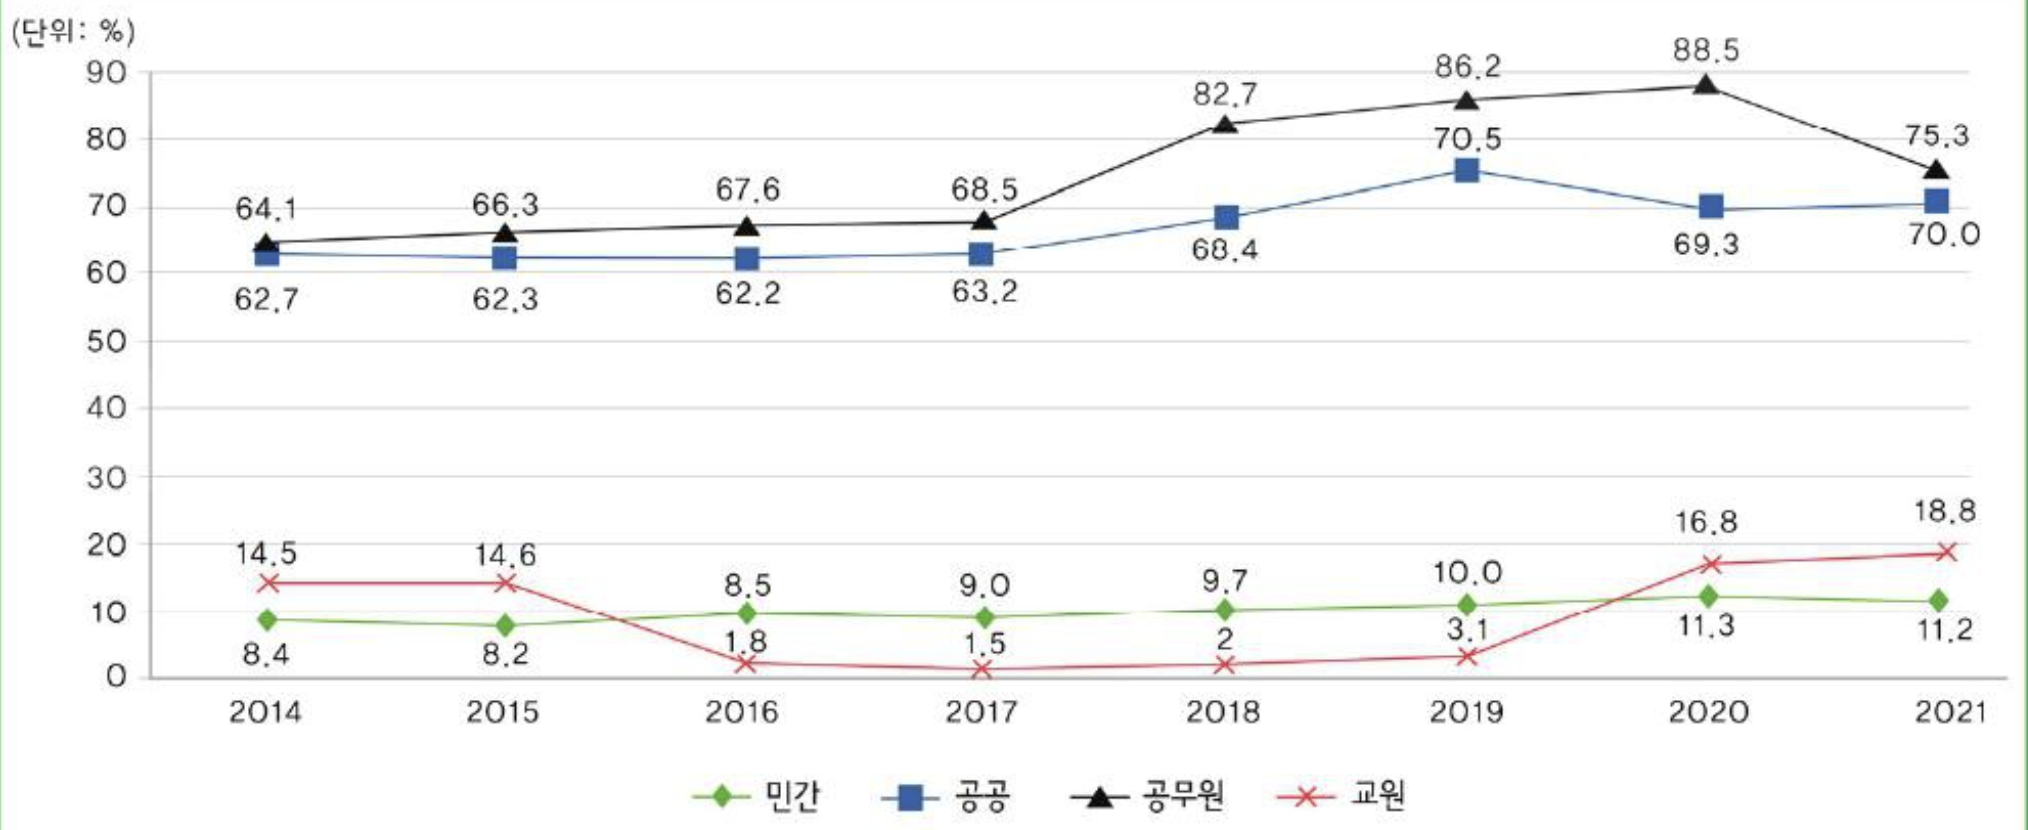
\includegraphics[width=.8\textwidth]{pic/부문별노조조직률변화추이.png}
    \caption{부문별 노조 조직률 변화 추이}
\end{figure}
\end{frame}

\begin{frame}
\centering
\begin{figure}
    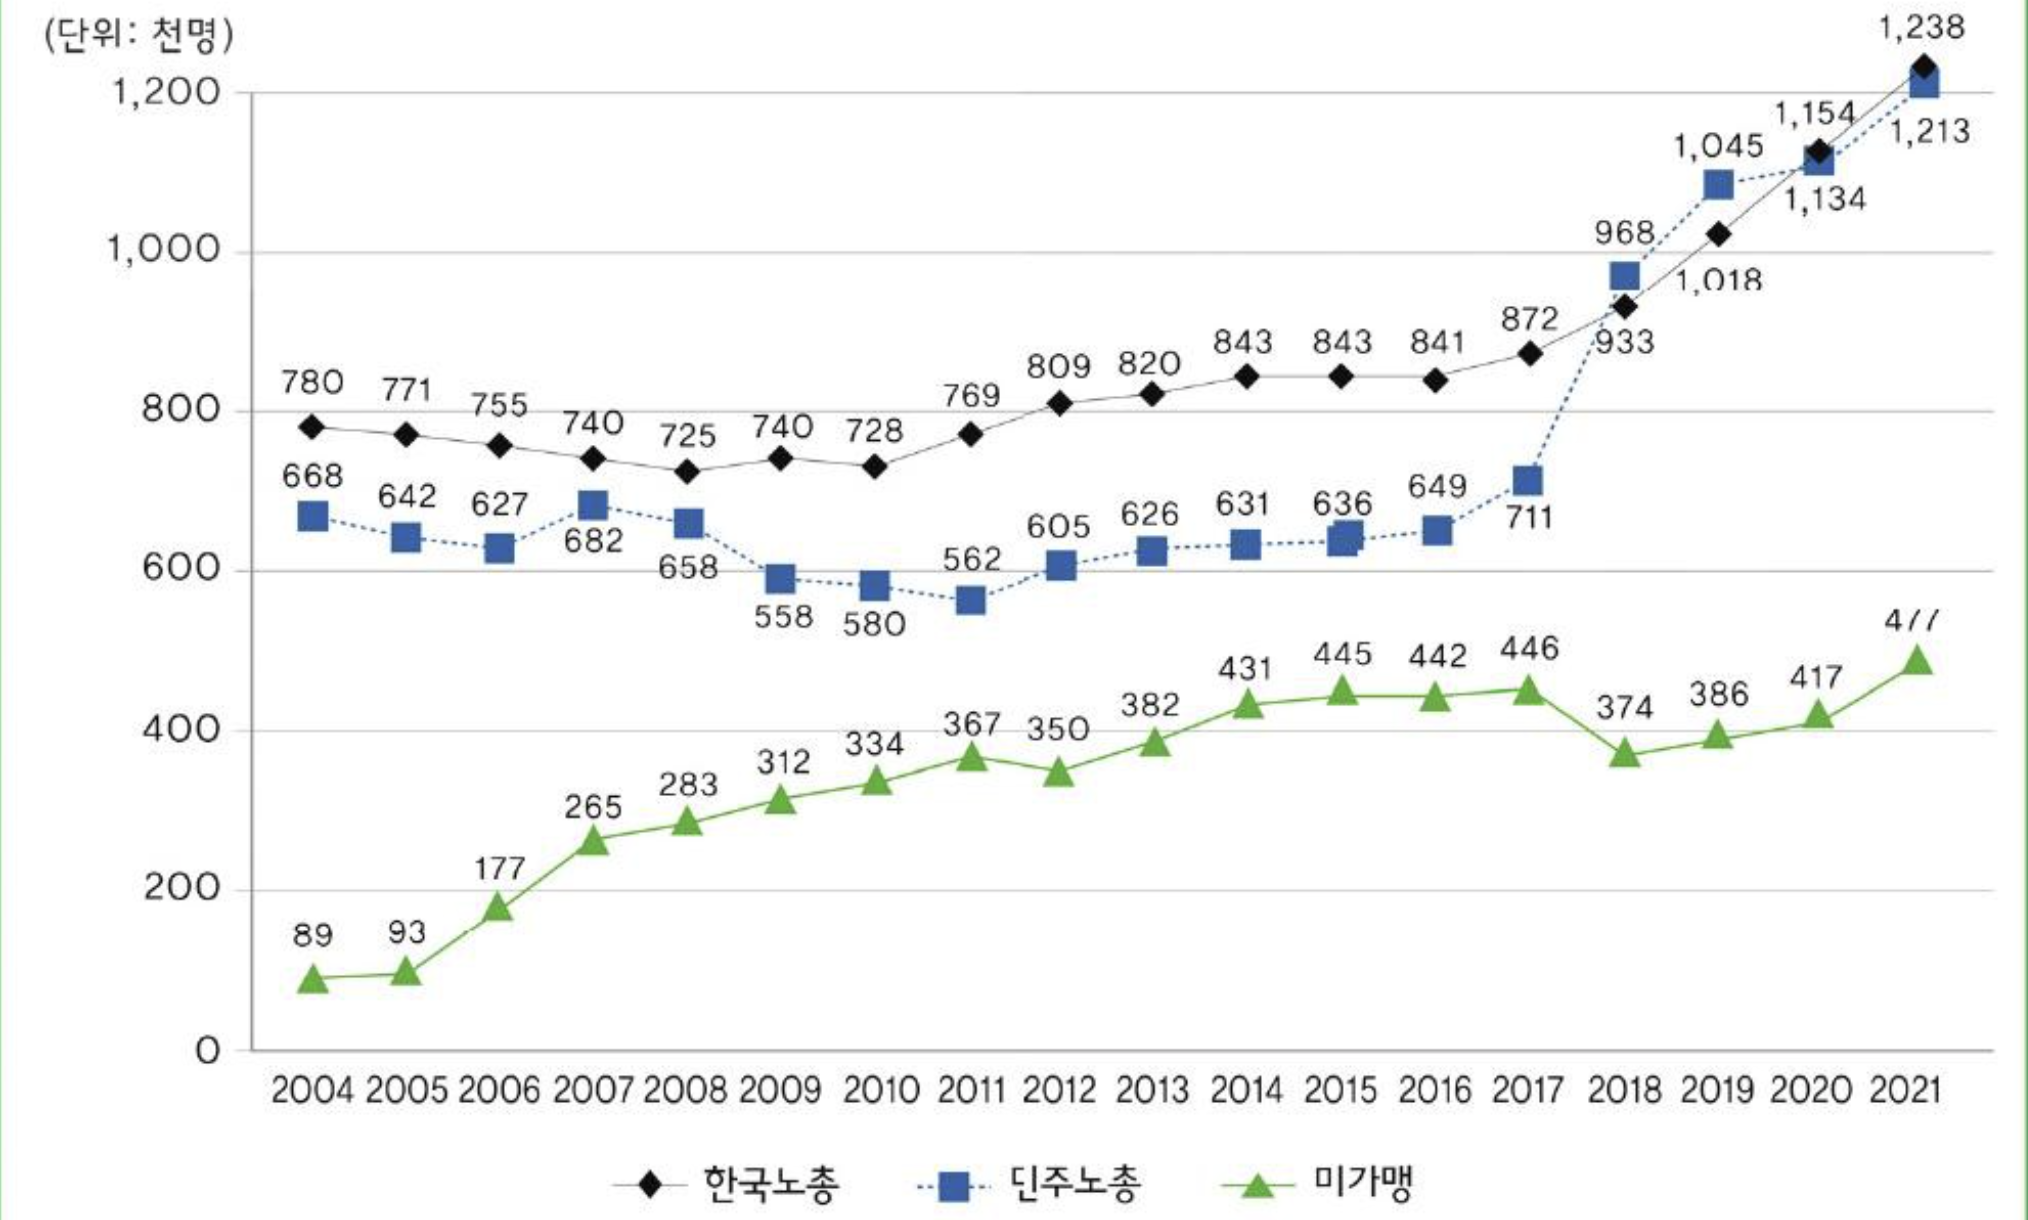
\includegraphics[width=.7\textwidth]{pic/상급단체별조합원수추이.png}
    \caption{상급단체별 조합원 수 추이}
\end{figure}
\end{frame}

\subsection{노조와 관련된 최근 이슈}

\begin{frame}{비정규직 노조}
    \begin{itemize}[<+->]
        \item 비정규 근로자는 고용불안과 상대적으로 열악한 근로조건 등으로 인해 노조에 대한 수요가 높음
        \begin{itemize}[<+->]
            \item 현실적으로 사용자의 보복을 우려해 노조의 설립·존속이 어려움
            \item 2021년 비정규직 노조 조직률은 3.3\%, 정규직 노조 조직률 18.4\%
        \end{itemize}
        \item 비정규직 노조의 특징  
        \begin{itemize}[<+->]
            \item 단체교섭의 확보를 위해 파업을 경험
            \item 약한 교섭력 (보조적·미숙련 업무 수행)
            \item 협상 상대방 모호
            \item 교섭단위와 조직단위의 불일치
        \end{itemize}
    \end{itemize}
\end{frame}

\section{경영자조직}

\subsection{경영자 조직의 구분과 국가별 형태}

\begin{frame}{}
    \begin{itemize}[<+->]
        \item 경영자들의 조직은 사업자조직과 사용자조직으로 구분
        \begin{itemize}[<+->]
            \item 사업자조직 (trade or business association): 경쟁, 관세, 대정부로비 등 기업경영상의 일반적인 문제를 다룸
            \item 사용자조직 (employers association): 기업경영상의 노동문제를 중점적으로 다룸
        \end{itemize}
        \item 사용자조직의 국가별 형태
        \begin{itemize}[<+->]
        \item 북유럽형 (스웨덴, 독일): 사용자 조직이 단체협상에 관여, 노사정협의체 등에서 영향력을 발휘함
        \item 동아시아형 (한국, 일본): 사용자 조직이 정부나 입법부에 대해 로비하거나 중앙에서의 노사정협의체에 참가, 회원 정보나 교육 훈련 서비스 등
        \item 미국형: 중앙 조직이 없음, 사용자 조직의 활동이 미약함
        \end{itemize}
    \end{itemize}
\end{frame}

\subsection{경영자조직의 역할}
\begin{frame}[allowframebreaks]{경영자조직의 주요 역할}
    \begin{itemize}[<+->]
        \item 정책참여 역할: 노동, 사회 및 경제정책들에 대한 사용자들의 입장을 정리하고, 사회적 협의기구 (예: 노사정위원회 등), 정부와 정당 등에게 의견을 개진하고 영향을 행사
        \begin{itemize}[<+->]
            \item 예: 비정규직 입법안에 대한 사용자측 주장을 대변
        \end{itemize}
        \item 단체교섭 역할: 단체교섭에 직접 참여 또는 이를 지원하는 활동을 의미.
        \begin{itemize}[<+->]
            \item 주로 산업교섭이나 전국단위 교섭시 다수의 사용자를 대표하여 단체교섭을 수행
            \item 예1: 금속산업노조와의 산별교섭에 참여하는 금속산업사용자협의회
            \item 예2: 일반적 권고나 지침, 자료 제공 및 조율 등을 통해 개별기업의 단체교섭을 지원
        \end{itemize}
        \framebreak\relax
        \item 분쟁대응 역할: 노조와의 분쟁에 대하여 상호지원, 파업기금을 통한 공동의 방어, 직장폐쇄를 통한 대응, 분쟁 조정과정에서의 사용자 대변 등의 활동
        \item 회원서비스 역할: 사용자조직의 회원에게 다양한 유형의 조사와 연구를 전담하고, 통계, 제도분석 등의 정보를 산출·제공. 또한 회원사에게 단체교섭이나 인적자원관리 등에 대한 기법, 노동자 숙련훈련 등의 교육훈련 서비스도 제공
    \end{itemize}
\end{frame}

\begin{frame}{한국의 주요 경영자 조직}
    \scriptsize
    \begin{table}
        \centering
        \resizebox{.8\textwidth}{!}{\relax
            \begin{tabular}{c|c|p{4cm}|p{7cm}}
\toprule
\textbf{단체명} & \textbf{설립년도} & \textbf{구성(회원사)} & \textbf{목적 및 활동} \\ \midrule
\textbf{한국경영자총협회} & 1970년 & 4,303개사 \newline (지방경총 회원사 포함) & 사용자의 이익대변, 협력적 노사관계 구축, 산업평화 도모, 기업의 인사노무관리 지원, 인사노무 관련 정보 제공, 국내외 교육연수 프로그램 운영 및 국제교류 협력 등 \\ \hline
\textbf{전국경제인연합회} & 1961년 & 약 500개사 (단체회원 포함) & 경제계, 특히 재벌의 관심사항, 경제전반에 걸친 회원사간 협의 및 국제경제 교류추진 등 \\ \hline
\textbf{대한상공회의소} & 1884년 & 73개 지방상공회의소 & 주요 경제현안 및 업계 실태에 관한 조사연구, 교육연수, 경제정책 정보제공 및 국제교류 협력 등 \\ \hline
\textbf{중소기업중앙회} & 1962년 & 23개 중소기업연합회, \newline  981개 조합 (단체 포함) & 중소기업의 애로파악, 조사·연구 및 정책건의. 인력지원, 글로벌화 지원사업 등 \\ \bottomrule
\end{tabular}

        }
        \\
        \raggedright\relax % 왼쪽 정렬
        \caption{한국 경영자조직의 현황}
    \end{table}
\end{frame}

\section{정부}

\subsection{정부의 역할}

\begin{frame}{정부의 주요 역할}
    \scriptsize
    \begin{table}
        \centering
        \resizebox{.8\textwidth}{!}{\relax
            \begin{tabular}{p{4cm}|p{8cm}}  % 열 너비 조정
\toprule
\textbf{역할} & \textbf{내용} \\ \midrule
\textbf{사용자 역할} & 정부는 공무원과 공공부문 근로자에 대한 사용자 역할 수행 \newline 공공부문의 비중이 커지는 상황에서 정부의 사용자 역할 중요 \\ \hline
\textbf{집단적 고용관계의 절차와 게임의 법칙 결정 역할} & 단체협상, 단체행동 등 집단적 고용관계 전반에 대한 원칙과 절차를 정립하는 역할 수행 \\ \hline
\textbf{개별고용관계에 대한 근로기준 설정 역할} & 인간 삶을 영위하는 데 필요한 최소 조건 (최저임금, 사회보장, 보험 등) 보호를 위해 법제화를 하거나 지원방안 마련 \newline 근로자가 최소한의 근로기준과 복지혜택을 보도둑 하는 역할 \\ \hline
\textbf{거시 경제적 역할} & 노동시장의 수요·공급 조정과 노동시장 안정 도모 및 인력의 취업 역량 함양 \newline 정부는 재정·금융정책 및 중앙은행의 금리정책 등을 적절하게 운영하여 노동시장의 안정 도모, 인력의 취업역량 개발 \\ \bottomrule
\end{tabular}

        }
        \\
        \raggedright\relax % 왼쪽 정렬
        \caption{정부의 주요 역할}
    \end{table}
\end{frame}

\subsection{정부 조직 현황}

\begin{frame}{정부의 주요 조직}
    \scriptsize
    \begin{table}
        \centering
        \resizebox{.8\textwidth}{!}{\relax
            \begin{tabular}{p{1.6cm}|p{4.4cm}|p{8cm}}
\toprule
\textbf{기관명} & \textbf{주요 연혁} & \textbf{주요 업무 및 조직} \\ \midrule
\textbf{고용노동부} & 
1963년 노동청 \newline
1981년 노동부 \newline
2010년 고용노동부 & 
주요업무: 노사관계, 근로기준, 산업안전보건, 고용정책, 고용서비스, 청년여성고용, 직업능력정책 및 국제협력 등 \newline
지방조직: 6개 지방고용노동청, 40개 지청, 고용센터 \newline
산하기관: 근로복지공단, 산업인력공단, 노사발전재단 등 11개 기관 \\ \hline

\textbf{노동위원회} & 
1953년 노동위원회법에 따라 설치 & 
성격: 노동관계의 안정과 발전을 위해 조정과 판정 업무를 독립적 수행, 준사법적 기관 \newline
주요업무: 부당해고 판정, 부당노동행위 및 부당노동행위에 대한 심판, 차별시정, 구제명령 \newline
조직: 중앙노동위원회, 12개 지방노동위원회 및 특별노동위 \\ \hline

\textbf{경제사회발전} \newline \textbf{노사정위원회} & 
1998년 노사정위원회 \newline
2007년 경제사회발전 노사정위원회 \newline
2018년 경제사회노동위원회 & 
기능: 노동정책 및 이와 관련된 경제 사회 정책 통합 논의 \newline
구성: 근로자, 사용자, 정부, 공익을 대표하는 위원으로 구성 \newline
조직: 상무위원회, 의제별 업종별위원회, 사무처, 노사정대표자회의 \\ \bottomrule

\end{tabular}

        }
        \\
        \raggedright\relax % 왼쪽 정렬
        \caption{정부의 주요 조직 현황}
    \end{table}
\end{frame}

%------------------------------------------------
\end{document}
%------------------------------------------------
